\documentclass[12pt,utf8]{beamer}

% Gute Einführung zu LaTeX-Beamer: http://www2.informatik.hu-berlin.de/~mischulz/beamer.html

%-----PARAMETERS-----

%Wichtige Standard Pakete!
%\usepackage[german]{babel}
\usepackage{ngerman}
\usepackage{xcolor}
\usepackage{graphicx}
\usepackage{subcaption}
\usepackage{tikz}


%Für den Header notwendig!
%\usepackage[percent]{overpic}

\usepackage{hyperref} % für korrekte Links

%Einbinden des Themes
\input{design_latex-template/beamerthemeFOSSAG.sty}


%Standard Angaben
\title{
	\hspace*{8cm}
	\includegraphics[scale=0.2]{resources/logo_500px.png}
	\newline
	FOSS-AG
}
\subtitle{Git}
\author{@chef\_excellence}
\institute[FOSS AG]{\textbf{F}ree and \textbf{O}pen \textbf{S}ource \textbf{S}oftware \textbf{AG}}


\date{\today}

%-----IMPLEMENTATION-----
\begin{document}
	\begin{frame}
		\titlepage
	\end{frame}

	\begin{frame}
		TODO: LICENSE
	\end{frame}

	\begin{frame}
		\frametitle{Was ist Git?}
		\begin{itemize}
			\item Version Control System
			\item erlaubt verteilte Softwareentwicklung
		\end{itemize}
	\end{frame}

	\begin{frame}
		\begin{figure}
			\begin{subfigure}[t]{0.3\textwidth}
				\centering
				\includegraphics[width=\textwidth]{resources/subversion.png}
				\caption*{\tiny{\cite{subversion}}}
			\end{subfigure}
			~
			\begin{subfigure}[t]{0.3\textwidth}
				\centering
				\includegraphics[width=\textwidth]{resources/git.png}
				\caption*{\tiny{\cite{git_logo}}}
			\end{subfigure}
			~
			\begin{subfigure}[t]{0.3\textwidth}
				\centering
				\includegraphics[scale=0.6]{resources/mercurial.png}
				\caption*{\tiny{\cite{mercurial}}}
			\end{subfigure}
		\end{figure}
	\end{frame}

	\begin{frame}
		\frametitle{Was macht Git anders?}
		\centering
		In a nutshell:\\
		\textbf{Snapshots statt Diffs}
	\end{frame}

	\begin{frame}
		\frametitle{Diffs}
		\begin{figure}[h]
			\centering
			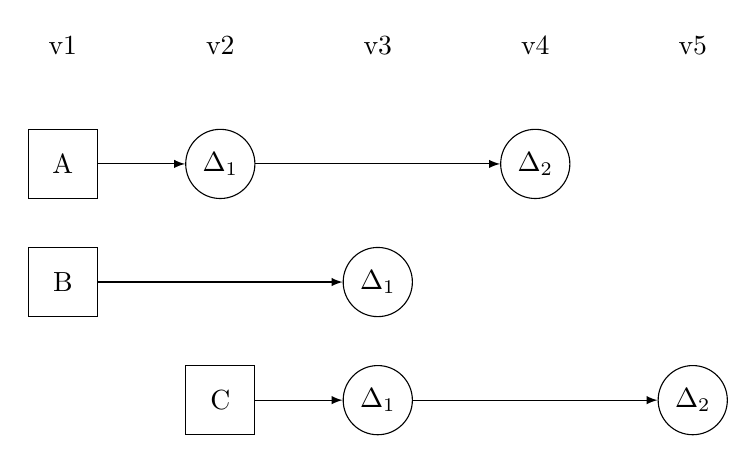
\begin{tikzpicture}
				\tikzstyle{version} = []
				\tikzstyle{file}=[draw, minimum size=25pt]
				\tikzstyle{diff}=[circle, draw, minimum size=25pt]
				\tikzset{edge/.style = {->,> = latex}}
				
				% versions
				\node[version](v1) at (0,1.5) {v1};
				\node[version](v2) at (2,1.5) {v2};
				\node[version](v3) at (4,1.5) {v3};
				\node[version](v4) at (6,1.5) {v4};
				\node[version](v5) at (8,1.5) {v5};
				
				% file A + diffs			
				\node[file](A)   at (0,0) {A};
				\node[diff](DA1) at (2,0) {$\Delta_1$};
				\node[diff](DA2) at (6,0) {$\Delta_2$};
				\draw[edge](A)   to (DA1);
				\draw[edge](DA1) to (DA2);
				
				% file B + diffs
				\node[file](B)   at (0,-1.5) {B};
				\node[diff](DB1) at (4,-1.5) {$\Delta_1$};
				\draw[edge](B)   to (DB1);
				
				% file C + diffs
				\node[file](C)   at (2,-3) {C};
				\node[diff](DC1) at (4,-3) {$\Delta_1$};
				\node[diff](DC2) at (8,-3) {$\Delta_2$};
				\draw[edge](C)   to (DC1);
				\draw[edge](DC1) to (DC2);
			\end{tikzpicture}
		\end{figure}
	\end{frame}
	
	\begin{frame}
		\frametitle{Snapshots}
		\begin{figure}[h]
			\centering
			\begin{tikzpicture}
			\tikzstyle{version} = []
			\tikzstyle{file}=[draw, minimum size=25pt]
			\tikzstyle{link} = [dash pattern=on 3pt off 3pt, draw, minimum size=25pt]
			\tikzset{edge/.style = {-,> = latex, dashed}}
			
			% versions
			\node[version](v1) at (0,1.5) {v1};
			\node[version](v2) at (2,1.5) {v2};
			\node[version](v3) at (4,1.5) {v3};
			\node[version](v4) at (6,1.5) {v4};
			\node[version](v5) at (8,1.5) {v5};
			
			% file A + diffs
			\node[file](A)   	at (0,0) {A};
			\node[file](A1)  	at (2,0) {A$_1$};
			\node[link](linkA1) at (4,0) {A$_1$};
			\node[file](A2)  	at (6,0) {A$_2$};
			\node[link](linkA2)	at (8,0) {A$_2$};
			\draw[edge](linkA1) to (A1);
			\draw[edge](linkA2) to (A2);
			
			% file B + diffs
			\node[file](B)   	 at (0,-1.5) {B};
			\node[link](linkB)	 at (2,-1.5) {B};
			\node[file](B1) 	 at (4,-1.5) {B$_1$};
			\node[link](linkB1)  at (6,-1.5) {B$_1$};
			\node[link](link1B1) at (8,-1.5) {B$_1$};
			\draw[edge](linkB) 	 to (B);
			\draw[edge](linkB1)  to (B1);
			\draw[edge](link1B1) to (linkB1);
			
			% file C + diffs
			\node[file](C)   	at (2,-3) {C};
			\node[file](C1)  	at (4,-3) {C$_1$};
			\node[link](linkC1)	at (6,-3) {C$_1$};
 			\node[file](C2) 	at (8,-3) {C$_2$};
			\draw[edge](linkC1)	to (C1);
			\end{tikzpicture}
		\end{figure}
	\end{frame}

	% Vorteile von Snapshots sind besonders stark, wenn es um Branching geht

	\begin{frame}
		\frametitle{Git ist schnell!}
		\begin{itemize}
			\item Geschwindigkeitsvorteil gegenueber vielen anderen VCSs
			\item Fast alle Operationen finden lokal statt und benoetigen keine Kommunikation mit einem Server
			\begin{itemize}
				\item Git-History durchsuchen
				\item auf ein alte Revision wechseln
				\item Aenderungen am Projekt commiten
			\end{itemize}
			\item[$\Rightarrow$] Kein Overhead durch Netzwerkkommunikation
		\end{itemize}
	\end{frame}
	
	\begin{frame}
		\frametitle{Support your local repo}
		\begin{itemize}
			\item Arbeiten und commiten auf lokaler Kopie des Projekts
			\item \texttt{git push} schiebt Aenderung auf den Server
			\item[$\Rightarrow$] erlaubt dezentralisiertes und lokales Arbeiten 
		\end{itemize}
	\end{frame}
	
	\begin{frame}
		\frametitle{Git vs. SVN}
		\begin{itemize}
			\item Aenderungen der Datei sind offline moeglich
			\item keine lokalen Commits moeglich
			\item \texttt{svn commit} = \texttt{git commit + git push}
		\end{itemize}
	\end{frame}

	\begin{frame}
		\frametitle{Die Dreifaltigkeit Gits}
		Jede Datei im Repository hat einen von drei Zustaende:
		\begin{itemize}
			\item Modified\\
				Die Datei wurde veraendert und entspricht nicht mehr der Version des momentanen Snapshots
			\item Staged\\
				Die Datei wurde fuer den naechsten Commit vorgemerkt und wird Teil des naechsten Snapshots
			\item Commited\\
				Die Datei wurde zum neuen Snapshot hinzugefuegt und ist in der lokalen Datenbank gespeichert
		\end{itemize}
	\end{frame}

	\begin{frame}
		\frametitle{Grundlegender Workflow}
		\begin{enumerate}
			\item Hack Hack Hack
			\item Hinzufuegen der veraenderten Dateien zur Staging Area\\
				\texttt{git add FILES}
			\item Erstellen des neuen Snapshots (lokal)\\
				\texttt{git commit -m COMMIT\_MESSAGE}
			\item Schiebe alle Aenderungen auf den Server\\
				\texttt{git push}
		\end{enumerate}
	\end{frame}

	\begin{frame}
	\frametitle{Statusbericht}
		\begin{itemize}
			\item Der Zustand der Dateien kann mit \texttt{git status -s} ueberprueft werden\\
			\item Zeigt zusaetzlich auch Dateien an, die nicht zum Projekt gehoeren (untracked files)
		\end{itemize}
	\end{frame}
	
	% NOTES
	%
	% - Grundlegende Funktionen von Git
	%   - Branches
	%   - Forks
	%   - Merge
	%
	% - Git Workflow
	%   - Arbeiten auf verschiedenen Branches
	%   - Arbeiten mit Pull/Merge Request
	%   - Issue-Tracker
	%
	% - Demonstrieren am Beispiel von Gitlab 
	% 
	
	\begin{frame}
		\bibliographystyle{plain}
		\bibliography{literatur}
		\addcontentsline{toc}{section}{\bibname}
	\end{frame}
	
\end{document}
